\documentclass[a4paper]{ctexart} %CTEX报告文章格式
\usepackage[top=3cm,bottom=2cm,left=2cm,right=2cm]{geometry} % 页边距
\usepackage{indentfirst}
\usepackage{graphicx}
\usepackage{fontspec}

\setlength{\parindent}{0em}
\CTEXsetup[format={\Large\bfseries}]{section}
% \CTEXsetup[name={,、},number={\chinese{section}}]{section}

\title{编译原理Lab2实验报告}
\author{Nosolution}
\date{}
\begin{document}
	\maketitle

	\section{截图}
	\begin{figure}[h]
	\centering
	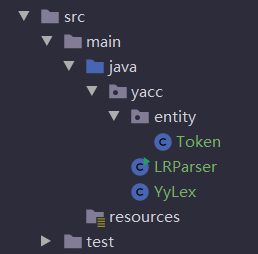
\includegraphics[scale=0.64]{../picture/yacc/源文件目录.png}
	\caption[l]{源文件目录}
	\end{figure}

	\begin{figure}[h]
		\centering
		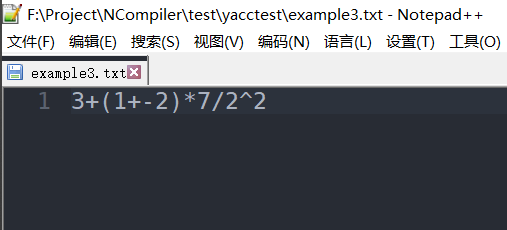
\includegraphics[scale=0.4]{../picture/yacc/输入1.png}
		\caption[l]{输入1}
	\end{figure}

	\begin{figure}[h]
		\centering
		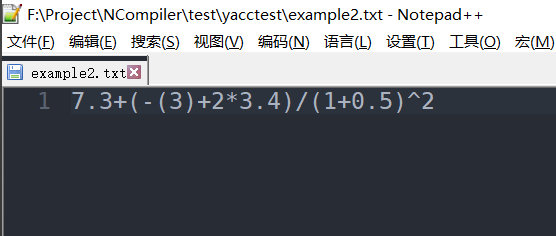
\includegraphics[scale=0.4]{../picture/yacc/输入2.png}
		\caption[l]{输入2}
	\end{figure}
	\newpage

	\begin{figure}[h]
		\centering
		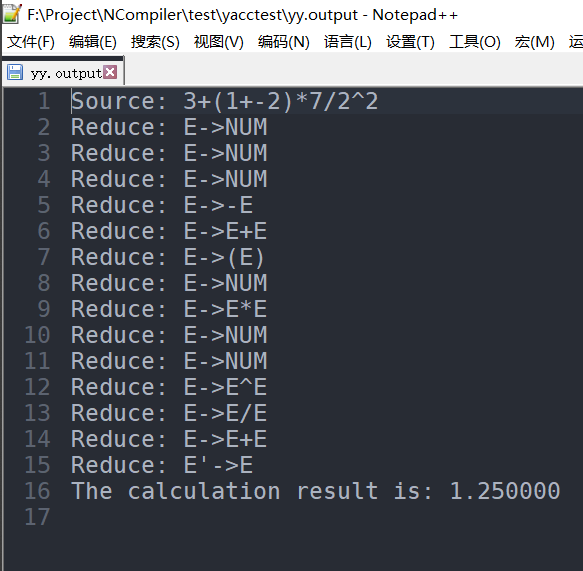
\includegraphics[scale=0.38]{../picture/yacc/输出1.png}
		\caption[l]{输出1}
	\end{figure}

	\begin{figure}[h]
		\centering
		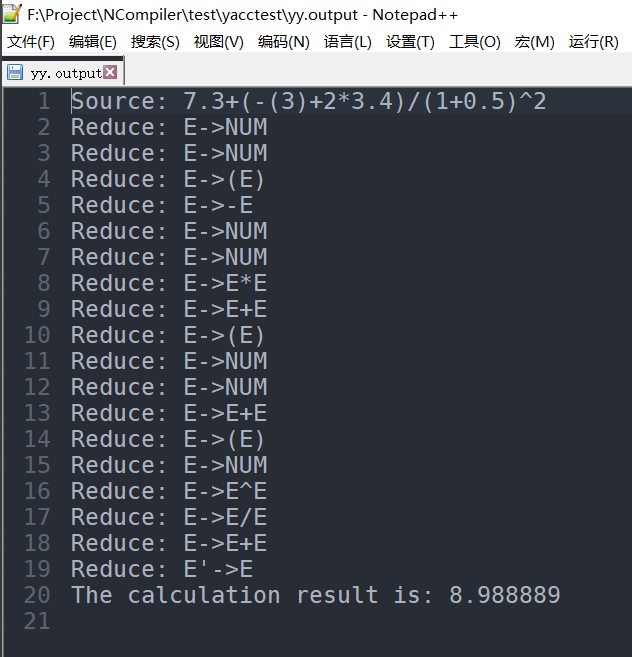
\includegraphics[scale=0.38]{../picture/yacc/输出2.png}
		\caption[l]{输出2}
	\end{figure}
	\newpage

	\begin{figure}[h]
		\centering
		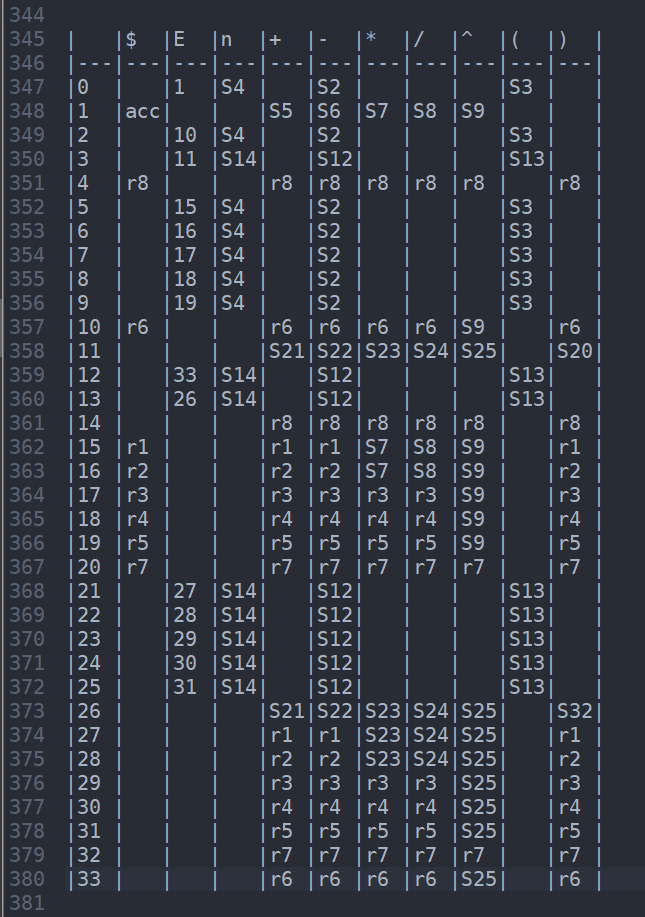
\includegraphics[scale=0.5]{../picture/yacc/LR分析表.png}
		\caption[l]{LR(1)分析表}
	\end{figure}


	\newpage
	\section{目标}
	使用LR(1)分析方法,仿照Yacc的生成代码,实现一个简单的计算器,以求对语法分析和Yacc更深入地了解。

	\section{项目描述}
	本次实验使用硬编码的实现方式,先手工推导出所有运算式的LR(1)项集和项集之间的转换关系,构造LR(1)预测分析表。再转化为合适的数据结构静态存储在代码中,运行代码对目标文件进行语法分析。

	\subsection{编译}
	使用\verb|mvn package|进行编译打包。

	如果成功,会在target目录下生成njyacc-1.0.jar和njyacc-1.0-jar-with-dependencies.jar文件

	\subsection{运行}

	直接运行: \verb|java -jar njyacc-1.0-jar-with-dependencies.jar <source path>|

	如果成功,输出文件为yy.output,格式:
	\begin{verbatim}
    Source: <source content>
    Reduce: ...
    Reduce: ...
    Reduce: ...
    ...
    The calculation result is: ...
	\end{verbatim}


	\section{基本思想和方法}
	基于LR(1)和有限状态机的方法,构造LR(1)项集后和转换关系后便得到确定性有限状态机,在每一个状态,根据向前看符号进行相应的状态转换,最终便可解析合法的符号串。

	\section{假设}
	使用的文法如下:
	\begin{verbatim}
        E->E+E
        E->E-E
        E->E*E
        E->E/E
        E->E^E
        E->-E
        E->(E)
        E->NUM
	\end{verbatim}
	其中\verb|NUM|代表数字,数值由lex进行解析。\\
	因为中缀表达式具有二义性,因而在文法上我附加了一些限制条件:

	\begin{itemize}
		\item 运算符的优先级: \verb|() > -|(单目)\verb| > ^ > */ > +-|
		\item  结合性: \verb|+-| 和 \verb|*/| 都是左结合的,\verb|^|是右结合的.
	\end{itemize}


	本次实现暂时没有错误处理,如果用户的输入存在语法错误,则程序会报错。

	\section{模型相关描述}

	我根据教学内容,将语法分析过程进行了建模,模型组件描述如下:
	\begin{itemize}
        \item{输入流} 由文法符号组成,能进行顺序访问的流
        \item{向前看符号} 指向输入流中下一个将被读取的文法符号
        \item{LR(1)分析表} LR(1)DFA的表表示形式,程序根据此表进行相应的动作
        \item{状态栈} 记录分析过程中的状态转移路径(规约后状态会被弹出)
        \item{符号栈} 记录所有尚未规约的文法符号
	\end{itemize}
	程序执行方式为循环执行,每次根据向前看符号选择对应的动作,并推进向前看符号。


	\section{重要的数据结构描述}

	\subsection{LR(1)分析表}
	按传统方式组织数据,每种状态(对应一个LR(1)项集)占有一行,对应所有可能输入的文法符号,并且不对字符和token进行区分。其中,使用正数代表移进动作,负数代表规约动作,0便意味着错误,程序会报错。\\
	表存储在一维数组中,按行顺序静态写入。

	\subsection{分析表查找}
	程序中\verb|yy_next|为分析表,查找时使用类似段式存储的思想,\verb|yy_next[base:offset]=next state|。其中\verb|base|即为使用当前状态作为索引在\verb|yy_base|表中的值,\verb|offset|即为输入文法符号的序号(已对所有可能的文法符号进行排序处理)。

	\subsection{产生式信息}
	\verb|yy_prod|数组存储所有产生式的相关信息长度为2*n+2。支持的产生式从序号1开始。2*i为产生式头部在文法符号中的排列序号,可以作为该文法符号的标识符;2*i+1为产生式体的长度,在规约时供算法使用。

	\section{核心算法描述}
	\subsection{lex解析}
	本实验中的lex程序十分简单,只负责判断本次读入的字符是不是数字,然后贪心查找至结尾,存储其值到\verb|yylval|变量中供语法分析器使用;否则直接返回本次读入字符。遇到空格时会不断跳过,遇到换行或者文件结尾会作为终止符号返回。
	\subsection{状态转移}
	状态转移使用状态栈和符号栈共同协作实现。\\
	状态栈的顶部状态为当前状态,当移进时压入新的状态,当规约时根据产生式体的长度弹出相应个数的状态以进行回溯,再压入产生式头部所代表的目标转移状态,等同于分层状态机中,下层状态机完成了全部转移,回到上层状态机进行一次移进。\\
	符号栈与状态栈保持动作协调,移进时压入当前向前看符号,规约时弹出产生式体所需要的符号,压入产生式头部

	\section{运行用例}

	\subsection{用例1}

	输入:
	\begin{verbatim}
	3+(1+-2)*7/2^2
	\end{verbatim}

	输出:
	\begin{verbatim}
	Reduce: E->NUM
	Reduce: E->NUM
	Reduce: E->NUM
	Reduce: E->-E
	Reduce: E->E+E
	Reduce: E->(E)
	Reduce: E->NUM
	Reduce: E->E*E
	Reduce: E->NUM
	Reduce: E->NUM
	Reduce: E->E^E
	Reduce: E->E/E
	Reduce: E->E+E
	Reduce: E'->E
	The calculation result is: 1.250000
	\end{verbatim}

	\subsection{用例2}

	输入:
	\begin{verbatim}
	7.3+(-(3)+2*3.4)/(1+0.5)^2
	\end{verbatim}

	输出:
	\begin{verbatim}
	Source: 7.3+(-(3)+2*3.4)/(1+0.5)^2
	Reduce: E->NUM
	Reduce: E->NUM
	Reduce: E->(E)
	Reduce: E->-E
	Reduce: E->NUM
	Reduce: E->NUM
	Reduce: E->E*E
	Reduce: E->E+E
	Reduce: E->(E)
	Reduce: E->NUM
	Reduce: E->NUM
	Reduce: E->E+E
	Reduce: E->(E)
	Reduce: E->NUM
	Reduce: E->E^E
	Reduce: E->E/E
	Reduce: E->E+E
	Reduce: E'->E
	The calculation result is: 8.988889	
	\end{verbatim}

	\section{出现问题及相关解决方案}
	上面所提到的较为完备的简单计算器总状态为34个,涉及总共10个文法符号,因此手写LR(1)项集需要花费的时间较多。并且因为需要频繁地回看之前写的状态来确定状态间的关系,也要求相当程度的细心和对这些项集的很高的把握程度。最终还是借助计算机等工具把项集和分析表写了出来。

	\section{个人评价}
	其一是LR(1)分析法确实是一个非常强大的工具,LR(1)项集封装了分层有限状态机中的层间的转换和推进的逻辑,个人感觉类似于NFA转换后的DFA,每一次状态转换都包含了多条产生式的推进。当构建好分析表后,只要知道下一个文法符号就可以选择正确的路径进行文法分析,即使是靠人也可以很轻松地依靠分析表来分析文法。\\
	其二是通过在二义性语法上提供额外的限制条件来解决冲突,可以很显著地减少LR(1)项集的个数,我尝试过将上述语法拆分成不同的产生式来显式地指定运算符的优先级和结合性,但很快发现项集的数量呈爆炸性增长,实在不适合人工推导。通过隐式指定优先级和结合性(等于为分析表中冲突项选择唯一的动作),就可以用不太多的项集完成该二义性语法的分析。\\
	其实本次实验的完成度不高,手工推导再硬编码实现文法分析的感觉并不好。如果能实现较为完整的yacc,由计算机来完成推导LR(1)分析表的工作,才算是更贴近编译原理这门课的教学目标。
	
\end{document}